\section{Overall Description}

\subsection{Product perspective}

\subsubsection{Scenarios}

\begin{enumerate}
    \item \textbf{User registration and first access} \\
    Alice is a cycling enthusiast who wants to keep track of her daily commutes and contribute to the community. She downloads the BBP application and selects the option to sign up. She inputs her personal details (username, email, and password). After validating her email via a link sent to her inbox, she logs in for the first time. The system welcomes her and shows her personal dashboard, which is currently empty of trips.

    \item \textbf{Recording a personal trip with statistics} \\
    Marco, a registered user, decides to go for a ride on Sunday morning. He opens the BBP app and presses the "Start Recording" button. He puts the phone in his pocket and enjoys his ride. Once he reaches his destination, he takes out his phone and presses "Stop". The system immediately processes the data and presents a summary of the trip, showing the total distance (45 km) and his average speed ($22~km/h$). Additionally, since the internet connection is available, the system automatically enriches this record with meteorological data from the area during that timeframe (Sunny, $25^{\circ}C$, Wind $10km/h$). Marco saves this trip to his personal archive.

    \item \textbf{Automated data collection and user confirmation (Positive Case)} \\
    Marco, a registered user, is riding his bike to work with the "Automated Mode" enabled in the settings. The system detects that his movement speed is compatible with a bicycle and automatically starts monitoring the sensors. During the ride, the smartphone's accelerometer detects a significant vertical jolt compatible with a pothole. When Marco stops biking, the system sends him a notification: "We detected a potential obstacle during your ride. Please verify." Marco opens the notification and sees a map with a pin on the location where the jolt occurred. He confirms that there was indeed a pothole. The system marks the information as valid and publishable.

    \item \textbf{Handling a False Positive in Automated Mode} \\
    Marco is using the BBP app in automated mode. While riding, he decides to jump off a curb to enter a park. The accelerometer detects a strong vibration and flags it as a potential anomaly. At the end of the ride, the system asks Marco to confirm a "Severe Obstacle" at that specific location. Marco recognizes the spot on the map and knows it wasn't a road defect, but his own action. He presses "Reject". The system discards the data, ensuring that no false information is added to the database.

    \item \textbf{Manual insertion of path status} \\
    Alice is walking her bike along a path she usually takes, but she notices that a section of the track is currently flooded and muddy due to recent rain. She decides to warn other cyclists immediately. She opens the BBP app, logs in, and selects the "Report Path" function. She manually selects the street segments on the map, sets the status to "Requires Maintenance" and adds a note about the mud. She sets the info as "Publishable" and submits it.

    \item \textbf{Browsing Trip History and Statistics} \\
    Marco wants to check his progress for the month. He opens the BBP app and navigates to the "My History" section. The system retrieves his list of past trips. He selects a trip from two weeks ago. The system displays the detailed map of the route he took, the weather conditions of that day, and his speed graph. Frank notices he is getting faster and closes the app with satisfaction.

    \item \textbf{Route planning and visualization (Unregistered User)} \\
    Marco is a tourist visiting the city and wants to go from the Central Station to the City Park by bike. He is not registered on BBP, but he can still access the "Explore" section. He enters his origin (Central Station) and destination (City Park). The system calculates possible routes and visualizes them on the map. It suggests two paths: Path A and Path B. The system highlights Path A as the best option because it has a higher score. Marco sees that Path B is shorter but marked as "Poor Condition", so he chooses Path A.

    \item \textbf{Automatic Activity Detection (Context Recognition)} \\
    Alice leaves her office and jumps on her bike to go home, forgetting to open the BBP app. She starts pedaling vigorously. After a few minutes, the system detects a sustained speed of 18 km/h and a movement pattern typical of cycling. The app sends a silent notification: "Cycling activity detected. Recording started". Alice arrives home and finds that her trip has been correctly tracked from the moment the system recognized the activity.

    \item \textbf{Publishing Private Data} \\
    Marco has recorded several trips in "Private" mode because he didn't want to share his location initially. However, he realizes that one of his routes covers a newly paved bike lane that isn't on the map yet. He goes into his "Trip History," selects that specific route, and clicks "Make Path Info Publishable". The system extracts the path quality data and updates the public inventory, allowing other users to benefit from this new information.

    \item \textbf{Viewing Path Details and Scores} \\
    Alice is planning a weekend ride and is looking at the map of her neighborhood. She sees a bike path marked in green. She taps on it to see the details. The system displays the "Path Score" ($4.8/5$) and the status "Optimal". She sees another path marked in yellow with a score of ($3.0/5$). By clicking on it, she reads that the status is "Medium" because of frequent tree roots. Based on this detailed information, she plans her route to avoid the yellow path.
\end{enumerate}

% Table 4: Scenarios Traceability Matrix
\begin{table}[h!]
    \centering
    \small
    \renewcommand{\arraystretch}{1.4} 
    \begin{tabularx}{\textwidth}{|c| >{\raggedright\arraybackslash}p{3.5cm} | >{\raggedright\arraybackslash}p{2.2cm} | >{\raggedright\arraybackslash}X|}
        
        \hline
        \textbf{ID} & \textbf{Scenario Title} & \textbf{Goals Covered} & \textbf{Shared Phenomena Covered} \\
        \hline
        
        S1 & User registration and first access & [G1] & [WM9] \\
        \hline
        
        S2 & Recording a personal trip with statistics & [G1], [G2], [G3] &  [MW1], [MW8], [WM6], [MW2] \\
        \hline
        
        S3 & Automated data collection and user confirmation (Positive Case) & [G5], [G6] & [WM2], [MW3], [WM4] \\
        \hline
        
        S4 & Handling a False Positive in Automated Mode & [G6] & [WM2], [MW3], [WM4] \\
        \hline
        
        S5 & Manual insertion of path status & [G4], [G7] & [WM3], [WM7] \\
        \hline
        
        S6 & Browsing Trip History and Statistics & [G1], [G2], [G3] & [WM8], [MW7], [MW1], [MW2] \\
        \hline
        
        S7 & Route planning and visualization (Unregistered User) & [G8], [G9] & [WM5], [MW4] \\
        \hline
        
        S8 & Automatic Activity Detection (Context Recognition) & [G10], [G1] & [WM2], [MW6] \\
        \hline
        
        S9 & Publishing Private Data & [G7], [G11] & [WM8], [WM7], [MW5] \\
        \hline
        
        S10 & Viewing Path Details and Scores & [G9] & [MW4], [MW5] \\
        \hline
        
    \end{tabularx}
    \caption{Scenarios Traceability Matrix}
    \label{tab:scenarios_traceability}
\end{table}
\clearpage

\subsubsection{Class Diagram}

The domain model distinguishes between RegisteredUsers, who track activities and report data, and UnregisteredUsers restricted to navigation. The central Trip entity records cycling history by aggregating GPSCoordinates and calculating TripStatistics, while linking to SensorAnomaly for automated defect detection and Weather Data for environmental context.

Path management relies on BikePathSegments, which maintain status and Obstacle history derived from user-submitted PathReports. These inputs determine the PathScore, a metric used alongside the external MapService to process user RouteRequests and generate optimized RouteResults, ensuring recommendations reflect the most current community-validated road conditions.

\begin{figure}[h]
    \centering
    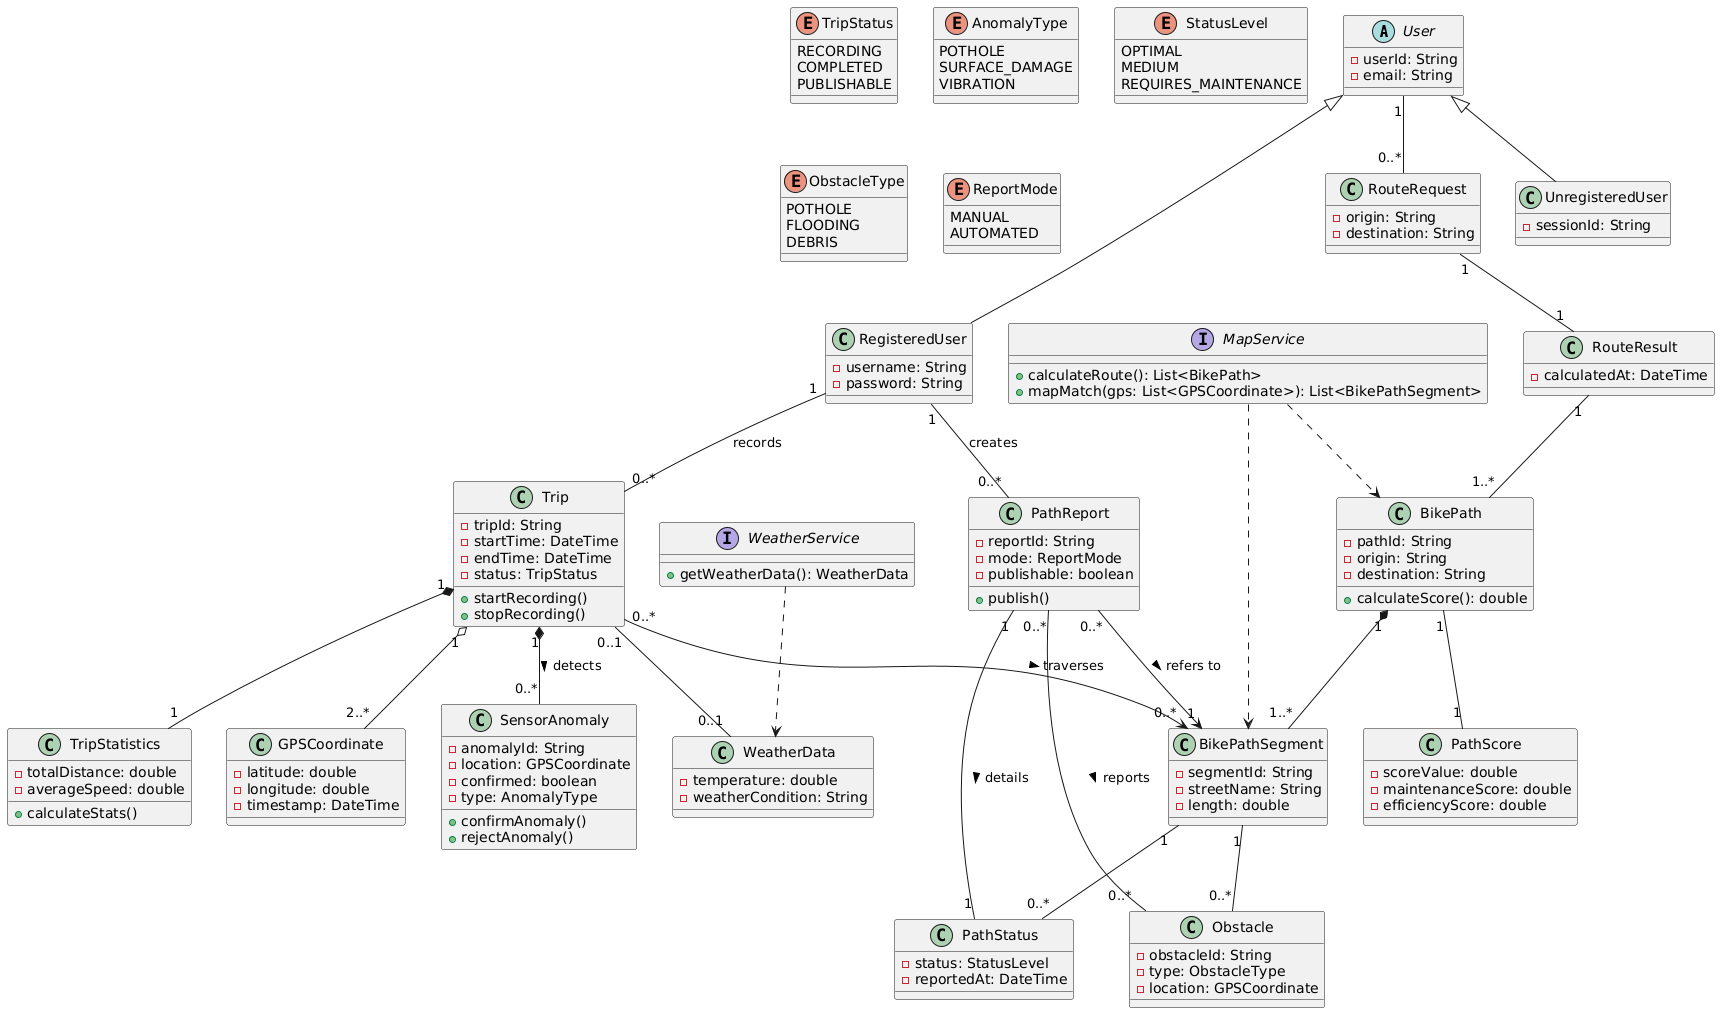
\includegraphics[width=\textwidth]{RASD/img/section2/class_diagram.png}
    \caption{Class Diagram}
    \label{fig:class_diagram}
    
\end{figure}
\clearpage

\subsection{Product functions}

\subsubsection{User Registration (Sign Up)}
This functionality allows Unregistered Users to create a personal account to access the system's full features. The user provides personal details such as username, email, and password. The system verifies the validity of the input data (e.g. ensuring the email is not already registered). Upon successful validation, the system creates a new account and stores the user's credentials.
\begin{figure}[H]
    \centering
    \label{fig:user_registration}
    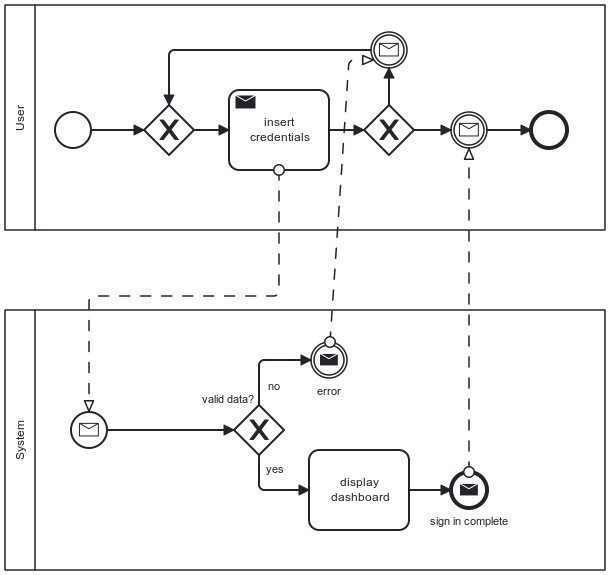
\includegraphics[width=\textwidth]{RASD/img/section2/diagram1.png}
     \caption{User Registration BPMN}
\end{figure}
\clearpage

\subsubsection{User Login}
This functionality grants Registered Users access to their personal area. The user inputs their credentials, and the system authenticates them against the database. If the authentication is successful, the user is redirected to their personal dashboard; otherwise, an error message is displayed.
\begin{figure}[H]
    \centering
    \label{fig:user_login}
    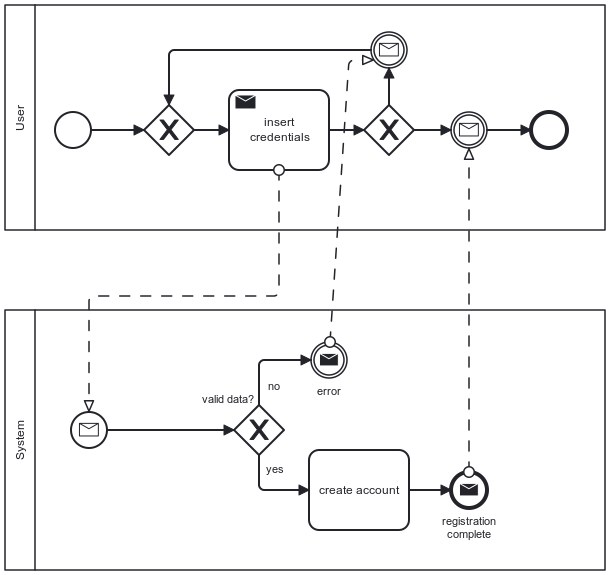
\includegraphics[width=\textwidth]{RASD/img/section2/diagram2.png} 
        \caption{User Login BPMN}
\end{figure}
\clearpage

\subsubsection{Record Personal Trip}
This functionality allows Registered Users to manually track their cycling activity. The user initiates the recording via the application interface. During the ride, the system continuously tracks the user's geolocation (GPS) and time. The recording continues until the user explicitly stops it, at which point the raw data is saved locally for processing.
\begin{figure}[H]
    \centering
    \label{fig:record_trip}
    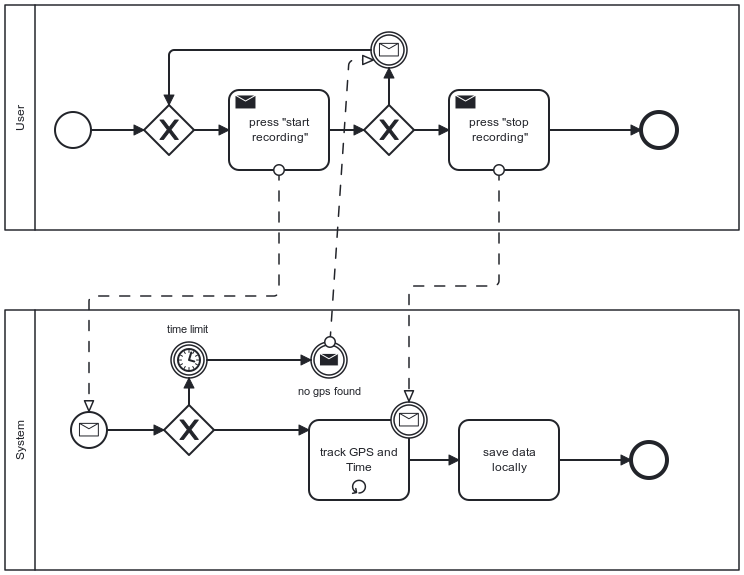
\includegraphics[width=\textwidth]{RASD/img/section2/diagram3.png}
    \caption{Record Personal Trip BPMN}
\end{figure}
\clearpage

\subsubsection{Trip Statistics \& Weather Enrichment}
Once a trip is completed, this functionality processes the raw data to calculate performance metrics such as total distance and average speed. Furthermore, the system connects to an External Weather Service to retrieve meteorological conditions, specific to the time and location of the trip. These details are then displayed to the user and archived in their history.
\begin{figure}[H]
    \centering
    \label{fig:trip_stats}
    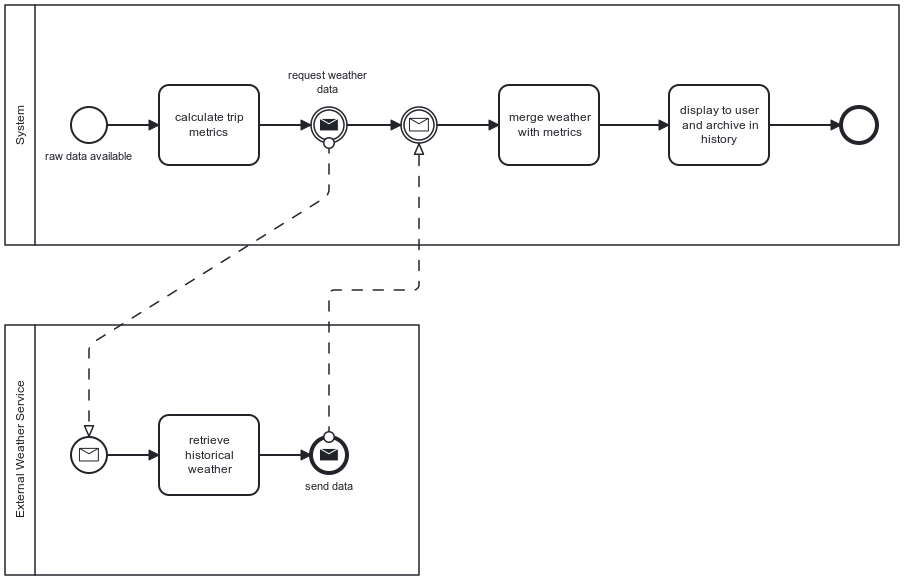
\includegraphics[width=\textwidth]{RASD/img/section2/diagram4.png}
    \caption{Trip Statistics \& Weather Enrichment BPMN}
\end{figure}

\subsubsection{Automated Data Collection}
This background functionality automatically detects when the user is cycling based on movement speed. Once activated, it collects data from the mobile device's sensors to identify road anomalies, such as potholes. Potential obstacles are flagged internally by the system for later verification.
\begin{figure}[H]
    \centering
    \label{fig:automated_data}
    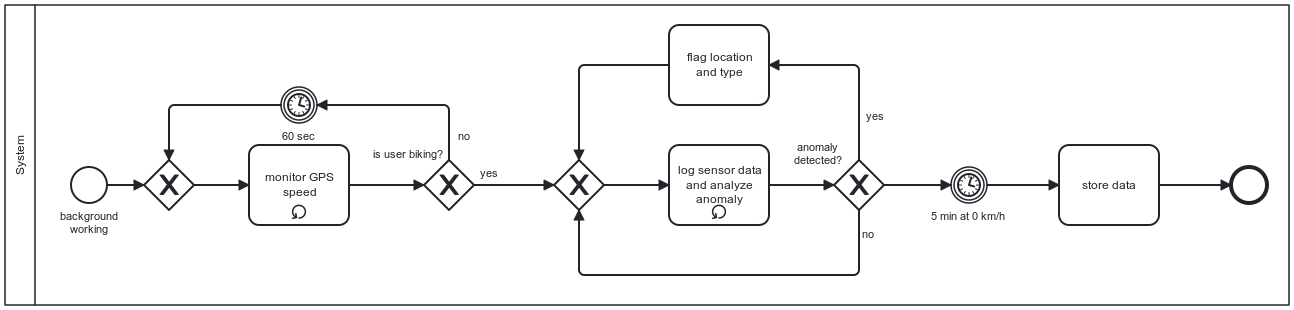
\includegraphics[width=\textwidth]{RASD/img/section2/diagram5.png}
    \caption{Automated Data Collection BPMN}
\end{figure}

\subsubsection{Verify \& Confirm Detected Data}
This functionality ensures the accuracy of automatically collected data. The system presents the user with a list or map of potential anomalies detected during the ride. The user must explicitly confirm if the anomaly was real or reject it (a false positive). Only confirmed data is stored as valid path information.
\begin{figure}[H]
    \centering
    \label{fig:verify_data}
    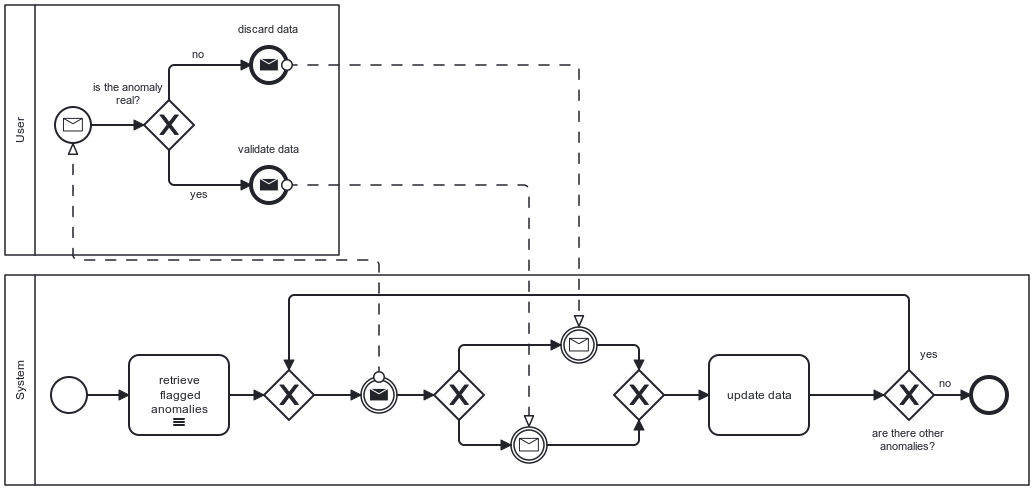
\includegraphics[width=\textwidth]{RASD/img/section2/diagram6.png} 
    \caption{Verify \& Confirm Detected Data BPMN}
\end{figure}

\subsubsection{Manual Path Reporting}
Registered Users can manually insert information about a specific path segment. The user selects a location on the map, specifies the status and indicates any obstacles. This data is saved to the user's personal records and can be optionally published.
\begin{figure}[H]
    \centering
    \label{fig:manual_reporting}
    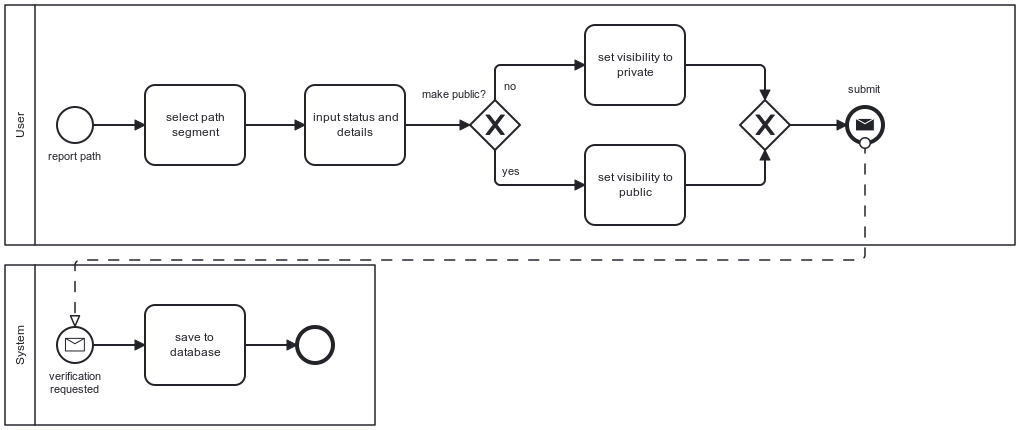
\includegraphics[width=\textwidth]{RASD/img/section2/diagram7.png} 
    \caption{Manual Path Reporting BPMN}
\end{figure}
\clearpage

\subsubsection{Publish Path Information}
This functionality allows Registered Users to contribute to the shared inventory. The user selects validated data (either manually reported or automatically confirmed) from their personal history and marks it as "Publishable". The system updates the public database, making this information available for other users' route planning.
\begin{figure}[H]
    \centering
    \label{fig:publish_info}
    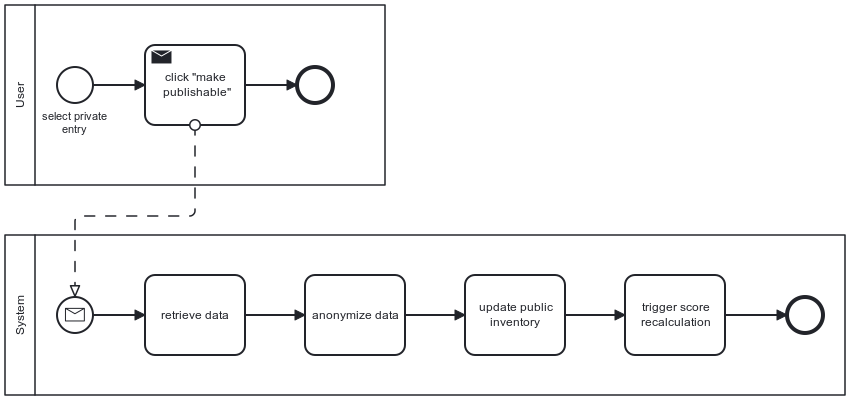
\includegraphics[width=\textwidth]{RASD/img/section2/diagram8.png} 
    \caption{Publish Path Information BPMN}
\end{figure}

\subsubsection{Route Planning \& Scoring}
This functionality allows any user (Registered or Unregistered) to find the best bike path between two points. The user inputs an origin and a destination. The system calculates available routes and assigns a score to each based on path status and efficiency. The results are visualized on a map, highlighting the highest-scored path.
\begin{figure}[H]
    \centering
    \label{fig:route_planning}
    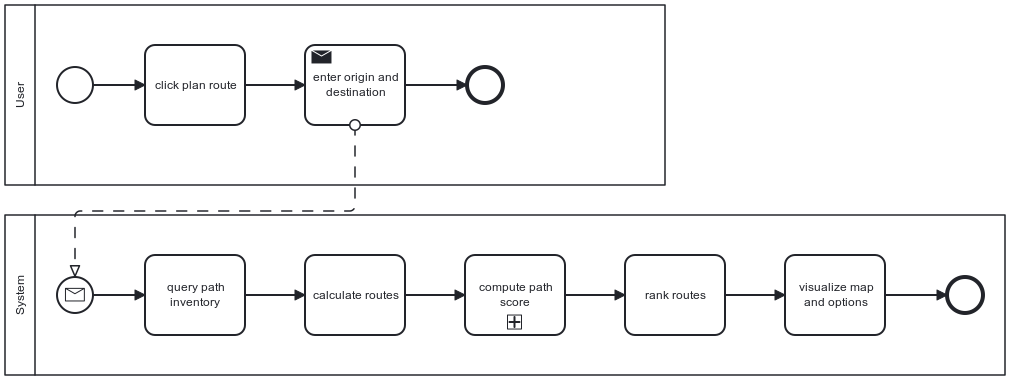
\includegraphics[width=\textwidth]{RASD/img/section2/diagram9.png}
    \caption{Route Planning \& Scoring BPMN}
\end{figure}
\clearpage

\subsubsection{View Statistics \& History}
This functionality enables Registered Users to access their personal archive of cycling activities. The user accesses the "History" section to view a chronological list of past trips. For each entry, the system provides a summary (date, distance, duration). By selecting a specific trip, the user can access detailed information, including the route map, performance charts (speed/elevation), and the associated weather conditions recorded at the time of the trip.


\begin{figure}[H]
    \centering
    \label{fig:view_stats}
    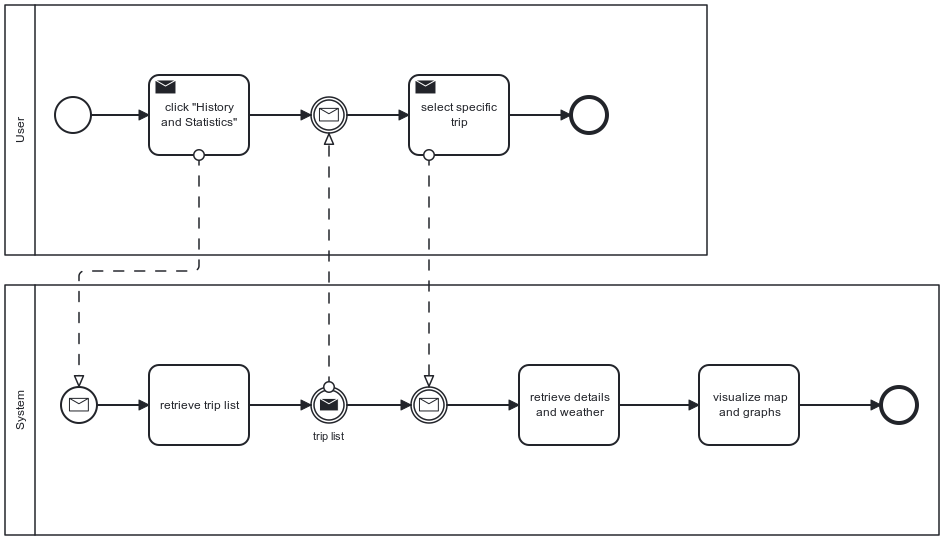
\includegraphics[width=\textwidth]{RASD/img/section2/diagram10.png} 
    \caption{View Statistics \& History BPMN}
\end{figure}
\clearpage
\subsection{Assumptions, dependencies and constraints}

\subsubsection{Domain Assumptions}
Domain assumptions are facts about the environment that are considered true for the system to function correctly. If these assumptions do not hold, the system may not be able to satisfy its requirements.

\begin{description}
    \item[\textbf{[D\_ASS1] GPS Availability:}] It is assumed that the Global Positioning System (GPS) signal is available and sufficiently accurate in the areas where the system is used to allow for meaningful path reconstruction.
    \item[\textbf{[D\_ASS2] Device Sensor Capability:}] It is assumed that the users' smartphones are equipped with a functioning accelerometer and gyroscope capable of detecting vibrations and orientation changes.
    \item[\textbf{[D\_ASS3] Device Placement:}] For the "Automated Mode" to function correctly, it is assumed that the user carries the smartphone in a position that allows the sensors to perceive road irregularities (e.g., firmly attached to the handlebar or in a pocket close to the body), rather than in a suspended bag where vibrations would be dampened.
    \item[\textbf{[D\_ASS4] Distinguishability of Speed:}] It is assumed that cycling speeds are sufficiently distinct from walking (too slow) and driving (too fast) to allow the system to infer cycling activity with a reasonable degree of confidence, triggering the automatic recording.
    \item[\textbf{[D\_ASS5] User Integrity:}] It is assumed that the majority of users provide truthful manual reports and confirmations regarding path conditions.
\end{description}

\subsubsection{Dependencies}
The BBP system relies on external systems and services to provide full functionality.

\begin{description}
    \item[\textbf{[DEP1] External Map Service:}] BBP does not create cartography from scratch. It depends on a third-party Map Provider (e.g., OpenStreetMap, Google Maps Platform) to render maps and provide the underlying road network topology for visualization.
    \item[\textbf{[DEP2] External Weather Service:}] The system depends on the availability and reliability of an external API to fetch real-time and historical meteorological data based on geolocation and timestamps.
    \item[\textbf{[DEP3] Mobile Data Connectivity:}] The system depends on the mobile network ($4G/5G$) to download map tiles, fetch weather data, and synchronize trip data with the server. However, core tracking features must be resilient to temporary loss of connectivity.
\end{description}

\subsubsection{Constraints}
Constraints are limitations imposed on the design and implementation of the solution.

\begin{description}
    \item[\textbf{[CON1] Regulatory \& Privacy:}] As the system collects sensitive geolocation data and personal history, it must strictly adhere to data protection regulations (e.g., GDPR). Private trips must remain inaccessible to other users unless explicitly published.
    \item[\textbf{[CON2] Hardware Heterogeneity:}] The system must function across a wide range of Android and iOS devices with varying sensor sensitivity and GPS hardware quality.
    \item[\textbf{[CON3] Connectivity Limitations:}] The application must support offline buffering. If a user cycles in a remote area without signal, the trip data and sensor logs must be stored locally and synchronized once connectivity is restored.
\end{description}